
\newpage
\section{Лекция 4}
\subsection{Метрики}
\begin{definition}
    \textbf{Метрика} $\rho$ на множестве $M$ --- это такая функция $\rho (x, y) \geqslant 0$, что 
    \begin{enumerate}
        \item $\rho (x, y) = \rho (y, x)$
        \item $\rho (x, y) > 0, x\neq y, \rho (x, x) = 0$ 
        \item $\rho (x, y) + \rho (y, z) \geqslant \rho (x, z)$
    \end{enumerate}
\end{definition}
Дана карта с расстояниями между городами.\\
$M$ = \{ города \}\begin{center}
    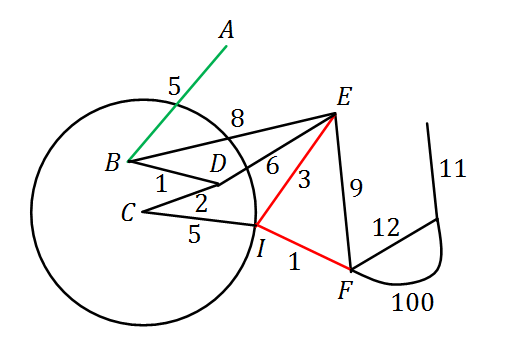
\includegraphics[scale=0.7]{l4_1.png}\end{center}
$\rho (A, B) = 5$\\
$\rho (E, F) = 4$ (минимальное расстояние из возможных)\\
\\
\begin{definition}
\textbf{Шар в метрическом пространстве.}\begin{center}
    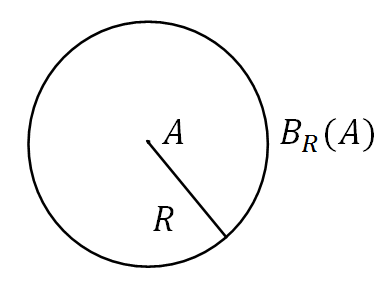
\includegraphics[scale=0.5]{l4_2.png}\end{center}
$B_R(A) = \{x | \rho(A, x) \leqslant R \}$ --- \textbf{шар} радиуса $R$ с центром в точке $A$.\\ 
$S_R(A) = \{x | \rho(A, x) = R \}$ --- \textbf{сфера} радиуса $R$ с центром в точке $A$.
\end{definition}
$B_5(C) = \{ C, B, D, I \}$ --- все точки, которые туда входят. \\
$S_5(C) = \{ I \}$ --- только те точки, которые лежат на окружности. \\
$B_{100}(C) = B_{50} (C) = M $ --- все множество. \\

\begin{notice}
    Метод наименьших квадратов --- приближение функции в смысле следующей метрики \begin{center} $M = \{f: X \rightarrow \mathbb{R} \}, X = \{ x_1, ..., x_n \}$\\ ~\\
        $\rho (f, y) = |\bar y - \bar f| = \sqrt{\sum\limits_{i=1}^n(y(x_i)-f(x_i))^2}$ \\
        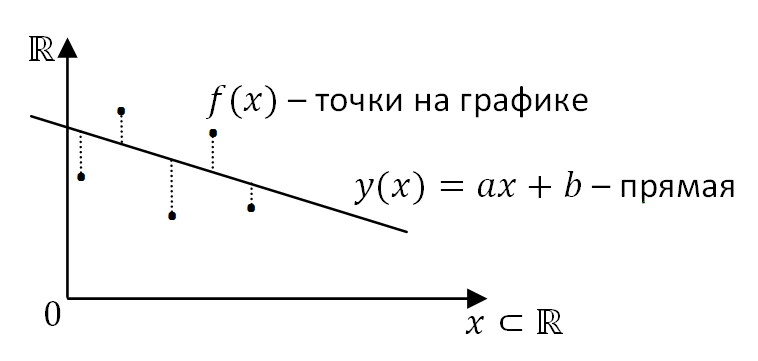
\includegraphics[scale=0.6]{l4_4.png}\end{center}
\end{notice}
\noindent \textbf{Пример 1.}\\
Найти такое метрическое пространство $M$, что\\ \\
$  
\left\{  
\begin{array}{lcl}  
B_5(x) \subset B_4(y) \\  
B_5(x) \neq B_4(y)\\
\end{array}   
\right.  
$
, где $x, y$ - две точки. \\ \\То есть доказать, что существует $c\in B_4(y), c\notin B_5(x)$.\begin{center}
    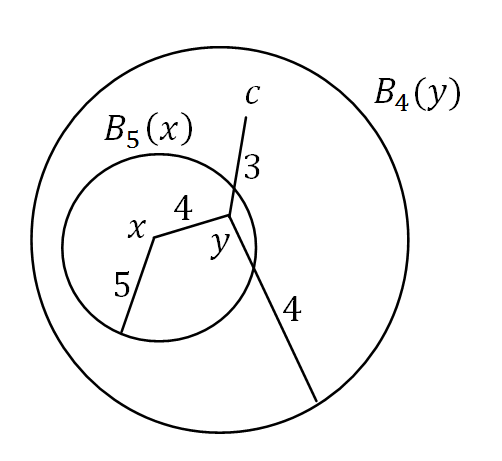
\includegraphics[scale=0.5]{l4_5.png}\\
    $\rho (x, y) = \rho(y, x) = 4$\\
    $\rho (y, c) = \rho(c, y) = 3$\\
    $\rho (x, c) = \rho(c, x) = 7$\\
    ~\\
    $B_5(x) = \{ x, y \}$\\
    $B_4(y) = \{x, y, c \} $\end{center}
То есть $B_5(x) \subset B_4(y)$.\\

\subsection{Нормы}
Вспомним определение линейного пространства.\\
Если на непустом множестве заданы две бинарные операции "+" и "умножение на число", числа из поля $F$, $\forall ~a,~b,~c\in V$ то\begin{enumerate}
    \item $a+(b+c) = (a+b)+c$
    \item $\exists~0: a+0 = 0+a = a$
    \item $\exists~ (-a): a+(-a) = 0$
    \item $a+b = b+a$
    \item $1\cdot x = x$
    \item $ (\mu \lambda)x = \mu(\lambda x)$
    \item $(a+b)\lambda = a\lambda + b\lambda$
    \item $(\mu + \lambda)a = \mu a + \lambda a$
\end{enumerate}
\begin{definition}
$V$ --- \textbf{линейное пространство} (векторное пространство), если выполнены 8 предыдущих аксиом и \begin{enumerate}
    \item $\forall \bar u, \bar v$: $\bar u + \bar v \in V$
    \item $\forall$ числа $\alpha \in$ $\mathbb{R}$, $\mathbb{C}$ $\alpha \bar u \in V$\\ 
    (или $\alpha \in F$ заданное поле, например, $F_2 = \{ 0, 1 \}$)\end{enumerate}
\end{definition}
\begin{definition}
Линейное пространство $V$ --- \textbf{нормированное}, если на нем задана такая норма \\$\nu : V \to$ $\mathbb{R}$ $\geqslant 0$, что\begin{enumerate}
    \item $\nu(\bar x) > 0$, $\bar x \neq \bar 0$, $\nu(\bar 0) = \bar 0$
    \item $\nu(\alpha \bar x) = |\alpha|\nu(\bar x)$
    \item $\nu(\bar x + \bar y) \leq \nu(\bar x) + \nu(\bar y)$ для $\forall x, y \in V, \forall \alpha$
\end{enumerate}
\end{definition}

\begin{notice}Из каждой нормы можно сделать метрику $\rho(\bar x, \bar y) = \nu(\bar y - \bar x)$.
\end{notice}
\textbf{Примеры норм:}\begin{enumerate}
    \item Манхэттенская норма (норма таксиста)\\
    (Можно ехать разными путями, но не по прямой)\begin{center}
        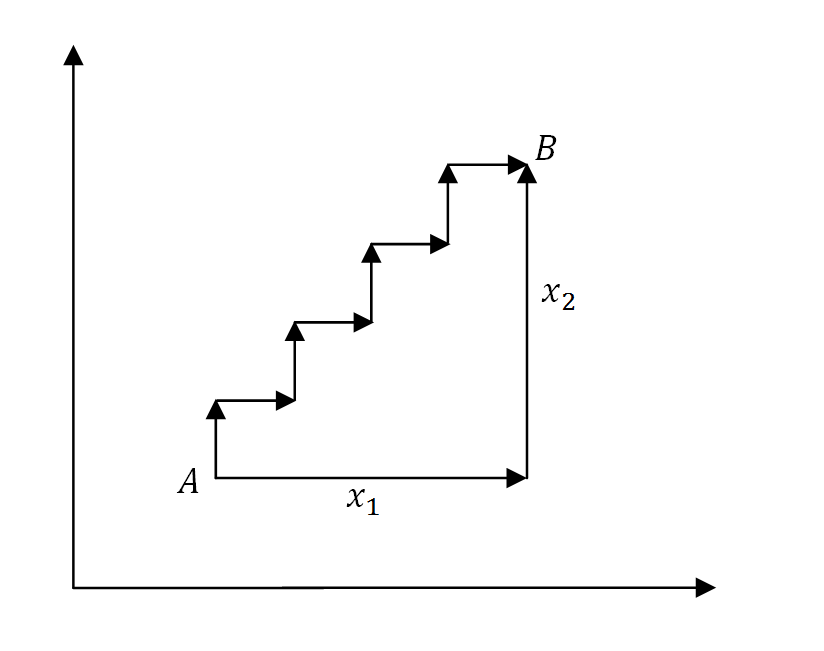
\includegraphics[scale=0.4]{l4_7.png}\end{center}
    \begin{center}$\nu_M(\bar x) = |x_1|+...+|x_n|$ в $\mathbb{R}^n$, где $\bar x = (x_1,..., x_n)$\end{center}
    \item Евклидова норма\\
    (Для приближения)
    \begin{center}
        $\nu_E(\bar x) = \sqrt{|x_1|^2+...+|x_n|^2}$ в $\mathbb{R}^n$\end{center}
    \item Норма максимума\\
    (Уменьшает ошибку по всем координатам)\begin{center}
        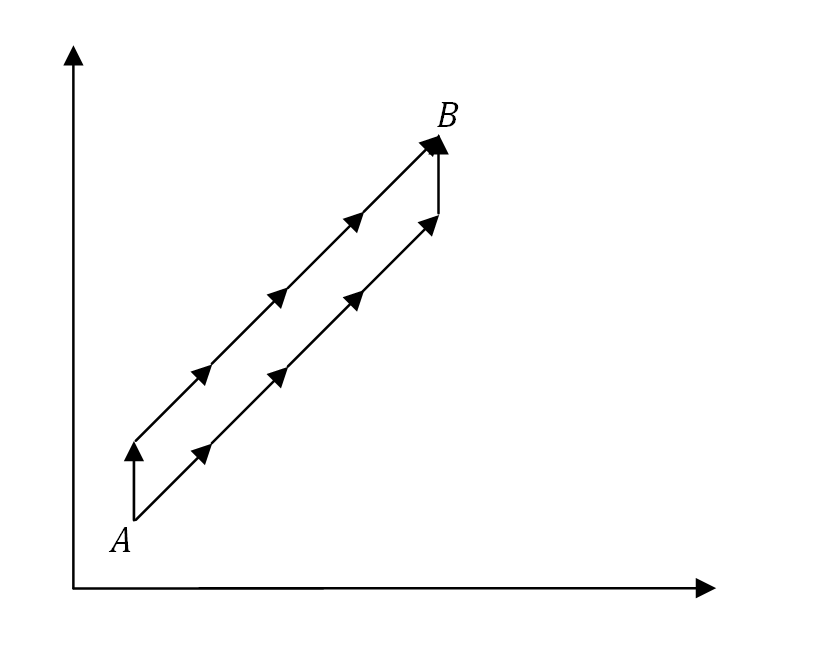
\includegraphics[scale=0.4]{l4_8.png}\end{center}
    \begin{center}
        $\nu_{max}(\bar x) = max\{|x_1|,...,|x_n|\}$ в $\mathbb{R}^n$\\\end{center}
    \item Норма Гёльдера
    \begin{center}$\nu_p(\bar x) = \sqrt[p]{|x_1|^p+...+|x_n|^p}$ в $\mathbb{R}^n$\\
        $\nu_1(\bar x) = |x_1|+...+|x_n| = \nu_M(\bar x)$\\ 
        $\nu_2(\bar x) = \sqrt{|x_1|^2+...+|x_n|^2} = \nu_E(\bar x)$\\
        $\nu_{\infty}(\bar x) = \underset{p \to \infty}{lim}\sqrt[p]{\sum\limits_{i=1}^n |x_i|^p}$\end{center}
    Если $|x_i| = max |x_i|$, то $\sqrt[p]{|x_i|^p} \to |x_i|$, получим:
    \begin{center}$\nu_{\infty}(\bar x) = max \{|x_1|,...,|x_n|\} = \nu_{max}(\bar x)$\end{center}
\end{enumerate}
\begin{statement}
    В нормированном пространстве $V$ верно:\begin{enumerate}
        \item $\forall \bar x, \bar y ~B_R(\bar x)$ равен $B_R(\bar y)$ (как геометрическая фигура).
        \item Шары $B_R(\bar x)$ и $ B_{\alpha R}(\bar x)$, $\alpha > 0$ подобны с коэффициентом подобия $\alpha$. 
    \end{enumerate}
\end{statement}
\begin{proof}
    \ 
    \begin{enumerate}
        \item Пусть $\bar v = \bar y - \bar x$, тогда \begin{center} $B_R(\bar y) = \bar v + B_R(\bar x)$\end{center}
        Ко всем точкам из $B_R(\bar x)$ прибавим одинаковый вектор $\bar v$.\begin{center}
            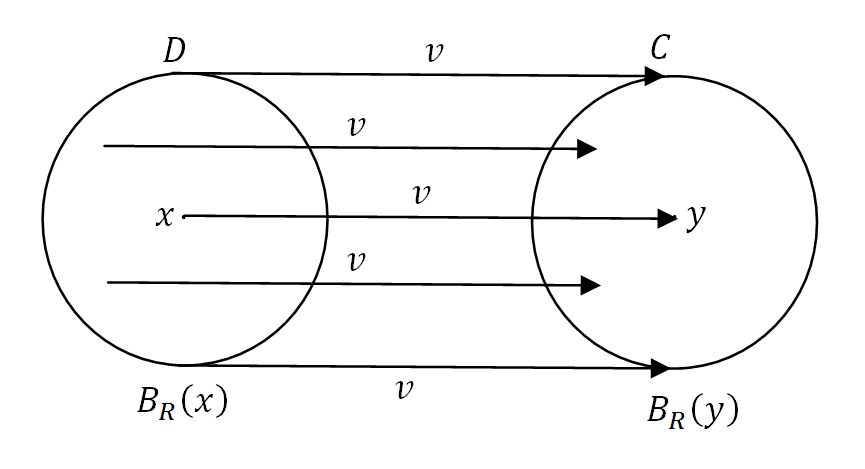
\includegraphics[scale=0.5]{l4_9.png}\\
            $C \in B_R(y) \Leftrightarrow \nu(C-y) \leqslant R$\\
            $\nu((C-(\bar y - \bar x))-\bar x) \leqslant R$\end{center}
        То есть, $D = C-(\bar y-\bar x) \in B_R(\bar x)$
        \item \ 
        \begin{center}$\nu(x D) = \cfrac{1}{\alpha}\nu(x C)$\\
        $D = x+xD = x+\cfrac{1}{\alpha}xC$\\
        $\rho(D, x) = \nu(x D) = \cfrac{1}{\alpha}\nu(C-x) = \nu(\cfrac{1}{\alpha}(C-x))$\\
        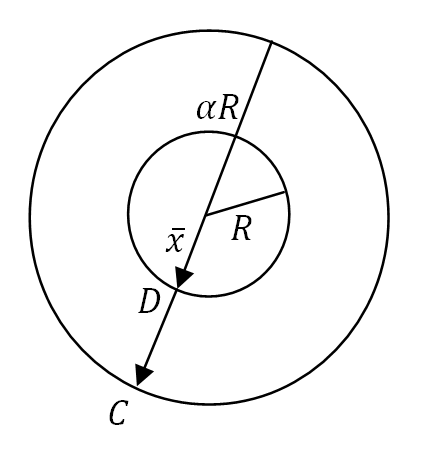
\includegraphics[scale=0.5]{l4_10.png}\\
        $C \in B_{\alpha R}(x) \Leftrightarrow \nu(C-x) \leqslant \alpha R$\\
        $\rho(D, x) = \nu(\cfrac{C-x}{\alpha}) \leqslant R$\end{center} То есть $D \in B_R(\bar x)$.
    \end{enumerate}
\end{proof}

\begin{notice}$\nu_p$ --- норма только при $p \geqslant 1$ (для невыпуклых --- неверно, не выполняется неравенство треугольника). 	$B^p = B_1(\bar 0)$ относительно $\nu_p$.\begin{center}
    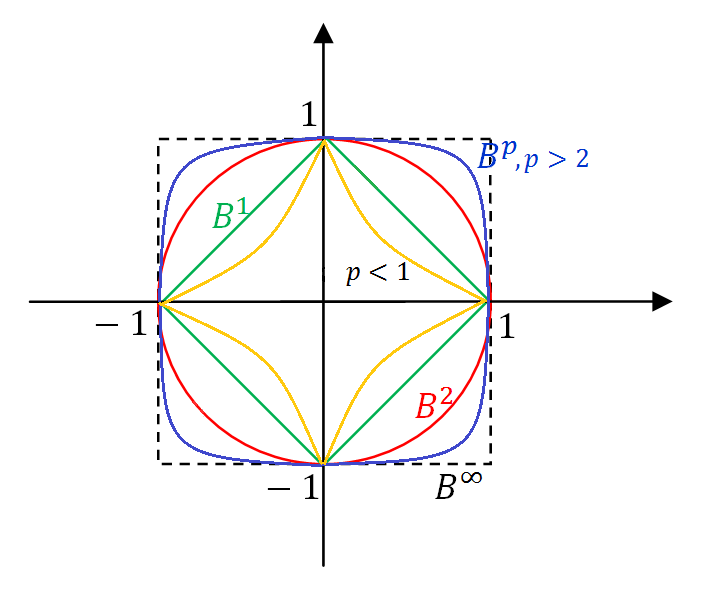
\includegraphics[scale=0.7]{l4_11.png}
    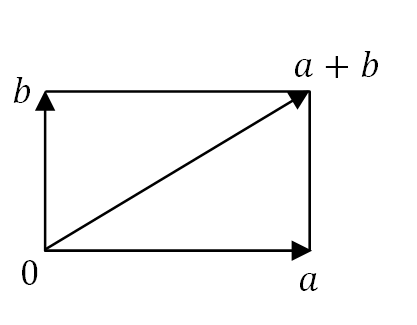
\includegraphics[scale=0.5]{l4_12.png}
\end{center}
\end{notice}
\textbf{Пример 2.}\\
Для каких $R_1, R_2$ возможно $B_{R_1}(x) \subsetneq B_{R_2}(y)$?\\
\\
Если $R_2 > R_1$ --- возможно (даже при $x = y$).\\
При $R_1 = 5, R_2 = 4$ --- возможно (из предыдущего примера).\\
Докажем, что при $R_1 > R_2$ это не всегда верно, а именно: при $2R_2 > R_1$ - верно, а при $R_2 \leqslant \cfrac{R_1}{2}$ --- нет.\\
Рассмотрим случай $2R_2 = R_1$. \begin{center}
    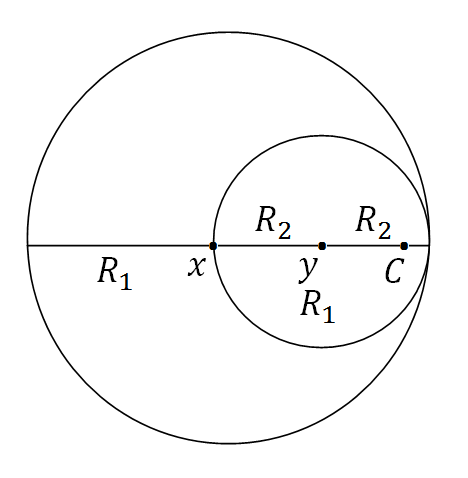
\includegraphics[scale=0.55]{l4_13.png}\end{center}
Тогда $B_{R_1}(x) = \{x, y, C\}$, $B_{R_2}(y) = \{x, y, C\}$, то есть $B_{R_1}(x) = B_{R_2}(y)$ --- множества совпадают, то есть уже не подходит.\\
\\
Рассмотрим случай, когда $R_1$ чуть меньше $2R_2$.\\
Тогда $B_{R_1}(x) = \{x, y\}$, $B_{R_2}(y) = \{x, y, C\}$, то есть $B_{R_1}(x) \subsetneq B_{R_2}(y)$ верно.\\
\\
Рассмотрим случай, когда $R_1$ чуть больше $2R_2$.\\
Тогда $B_{R_1}(x) = \{x, y, C\}$, $B_{R_2}(y) = \{x, y, C\}$, то есть, $B_{R_2}(y) \subseteq B_{R_1}(x)$, значит не подходит.
\begin{definition}
    Линейное пространство называется \textbf{евклидовым пространством}, если на нем задано скалярное произведение $g(x, y)$:\begin{enumerate}
        \item $g(x, y) = g(y, x)$
        \item $g(x_1+x_2, y) = g(x_1, y)+g(x_2, y)$
        \item $g(\lambda x, y) = \lambda g(x, y)$
        \item $g(x, x) \geqslant 0, g(x, x) = 0 \Leftrightarrow x = 0$
    \end{enumerate}
\end{definition}
В евклидовом пространстве есть стандартная норма $\parallel x \parallel = \sqrt{g(x, x)}$. 
$L_2[0, 1]$ --- множество функций, квадрат которых интегрируем по Риману.\\
$(f, g) = \int\limits_0^1 f(x) \overline{g(x)}\,dx$\\
$\parallel f \parallel_2 = \sqrt{\int\limits_0^1 |f(x)|^2\,dx}$\\
\\
$x_n \to x$ $\textbf{сходится по норме}$ $\nu(x)$, если $\forall \varepsilon > 0 ~ \exists N(\varepsilon)~$, что $\forall n > N(\varepsilon)$ верно $~\nu(x_n - x) < \varepsilon$.\\ \\
\textbf{Пример 3.}\\
Является ли нормой на множестве непрерывно дифференцируемых функций $C^1[a, b]$ следующее выражение: \begin{center}$\mu(f) = \underset{a \leqslant x \leqslant b}{max}(|f(x)|+|f'(x)|)$ ?\end{center}
Да, так как выполняются все свойства нормы.\begin{enumerate}
    \item $\mu(f) > 0$
    \item $\mu(\lambda f) = \lambda \mu(f)$
    \item $\mu(f+g) = max(|f+g|+|(f+g)'(x)|)$\\
    $\mu(f)+\mu(g) = max(|f|+|g|+|f'|+|g'|)$\\
    А так как $|f+g|\leqslant |f|+|g|$, то выполняется неравенство треугольника \\$\mu(f+g) \leqslant \mu(f) + \mu(g)$.\end{enumerate}
\textbf{Пример 4.}\\ Следует ли из сходимости по норме $\parallel f \parallel = \underset{a \leqslant x \leqslant b}{max} |f(x)|$ сходимость по $\mu(f)$, где \begin{center}$\mu(f) = \underset{a \leqslant x \leqslant b}{max}(|f(x)|+|f'(x)|)$ ?\end{center} Верно ли обратное?\\ \\
Докажем, что $f_k(x) \overset{\parallel f \parallel}{\rightarrow} f(x)$ и $f_k(x) \nrightarrow$ по $\mu(f)$.
\begin{center}
    $f = x, f' = 1$\\
    $f_k = \cfrac{1}{k}sin(xk^2)+x$\\
    $|f-f_k| \leqslant \cfrac{1}{k} |sin(xk^2)| \leqslant \cfrac{1}{k} \to 0$, то есть, сходится по норме.\\
    $f_k' = 1+k \cdot cos(xk^2)$\end{center}
$max \{|f(x)-f_k(x)|+|f'(x)-f_k'(x)|\} = max \{|\cfrac{1}{k}sin(xk^2)|+|1-1-k\cdot cos(xk^2)|\} \to \infty$, то есть, не сходится по $\mu(f)$.\\ \\
Обратное утверждение верно. При сходимости по $\mu(f)$ получим, что $|f(x)-f_k(x)|\to 0$, то есть сходится по норме.\\ \\
\subsection{Домашнее задание 4}\begin{enumerate}
    \item
    $B(x, y) = \{x^2+axy+4y^2 \leqslant 1\}$\\
    При каких $a$ на множестве $\mathbb{R}^2$ существует норма $\nu$ такая, что $B(x, y)$ --- единичный шар относительно нее? \\Найдите в этом случае
    \[\nu \begin{pmatrix}
    2 \\
    1\\
    \end{pmatrix}\]
    \item
    Будет ли метрикой на $\mathbb{R}$ функция $\rho(x, y) =$\begin{enumerate}
        \item $|x^2-y^2|$
        \item $sin(x-y)$
        \item $|e^x-e^y|$
    \end{enumerate}
    \item
    Существует ли убывающая последовательность непустых замкнутых ограниченных множеств с пустым пересечением (в произвольном метрическом пространстве)?
    \item
    Доказать, что шар в нормированном пространстве является выпуклым множеством. То есть доказать, что если $x, y$ принадлежат шару, то и весь отрезок $[x, y]$ принадлежит шару.\end{enumerate}